Virtual Arena is the application that Visual Solutions has created to do visual collaboration\cite{VirtualArena}. It supports one-to-one, one-to-many and many-to-many collaborative scenarios. The application uses a \gls{mcu} that acts as a media server. With this server Virtual Arena can support a lot more incoming and outgoing streams than in a simple peer-to-peer scenario. It also applies mitigation strategies for scenarios with limited bandwidth. Without going into too much detail of how the application is actually put together the main setup looks something like this: 
\\
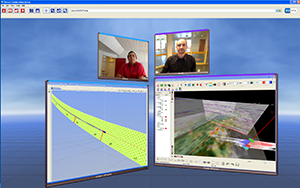
\includegraphics[scale=0.6]{virtualarena.png}
\\
\\

\subsection{Signaling}
Virtual Arena uses a proprietary way of doing signaling over RTCP.

Communication between peers and the media server is done by opening up ports in the firewall to listen for incoming tcp and udp connections. The media server can receives incoming streams and mix it in with the other streams and forward it to all the other peers. All the streams are identified using an SSRC.


\subsection{Transport layer}
Raw RTP stream over UDP.

\subsection{Media}
Speex for audio and theora for video.

\subsection{Security}
While \gls{wrtc} provides security such as \gls{dtls} on top of \gls{srtp}, Virtual Arena only uses raw \gls{udp} streams because nothing more is needed. It operates in a closed business environement, so transport level encryption is not needed, because unidentified peers are not allowed inside the network anyways.  The closed environment makes technologies like \gls{ice}, \gls{dtls}, and {srtp} unnecessary.

\subsection*{Summary}


Virtual Arena